%% IEEEtran manuscript. Compile on Overleaf (pdfLaTeX) or locally with a TeX
%% distribution. Figures are in paper/figures/ (relative path: figures/...).
\documentclass[journal]{IEEEtran}
\usepackage[utf8]{inputenc}
\usepackage[T1]{fontenc}
\usepackage{graphicx}
\usepackage{booktabs}
\usepackage{amsmath}
\usepackage{url}
\graphicspath{{figures/}}

\begin{document}

\title{Cross-Biome Deforestation Detection with a EuroSAT Transfer
Classifier: Domain Shift, Label-Free Adaptation, and a Spectral-Index Baseline}

\author{Joshua Anojulu% co-author / mentor to be added before submission
\thanks{J.~Anojulu is with the University of North Texas, Denton, TX, USA (e-mail: joshanojulu@gmail.com).}%
\thanks{Code and data: \url{https://github.com/Joshua-Anojulu/satellite-deforestation-classifier}}}

\maketitle

\begin{abstract}
We fine-tune a ResNet50 on EuroSAT to 98.26\% test accuracy (macro-F1 0.982) and
show that a 13-band multispectral variant of the same model gains nothing
(98.22\%): RGB saturates the benchmark on its own. We then ask what that accuracy
buys outside Europe. We apply the classifier to two-date Sentinel-2 imagery (2016 and
2024) at eight deforestation frontiers across three biomes and five countries
(Amazon: Rond\^onia, S\~ao F\'elix do Xingu, Mato Grosso; Indonesian peat/palm:
Riau; Congo Basin: Tshopo, Mai-Ndombe; dry forest: Santa Cruz, Gran Chaco), and we
score the resulting Forest$\rightarrow$non-Forest change against the Hansen Global
Forest Change record. The classifier loses most of that accuracy outside Europe.
Without radiometric correction it labels 72\% of a Rond\^onia rainforest scene as
water, and per-channel moment matching repairs that. Even after matching, it
collapses at three of the eight sites, returning zero or near-zero correct
detections at both Congo Basin sites and at Gran Chaco, on composites that our
diagnostics show to be cloud-free. Recomputing BatchNorm statistics on each target
scene (AdaBN) costs one label-free forward pass and no retraining, and it removes
all three collapses: at Tshopo, F1 climbs from 0.001 to 0.397 and precision from
0.02 to 0.70, with non-overlapping bootstrap intervals. AdaBN gives the steadiest
detector across biomes (mean F1 $0.250\pm0.130$) without giving the strongest. A
classical NDVI-difference baseline with a per-scene Otsu threshold posts the highest
mean F1 ($0.337\pm0.213$) and wins five of eight sites, yet it fails at Santa Cruz,
recovering 2 of 383 loss cells. The plain CNN trails NDVI across sites (Wilcoxon
$p{=}0.055$, $n{=}8$). No detector wins at all eight. If you deploy such a tool,
robustness across biomes will matter more to you than peak in-biome F1, and an RGB
CNN carried into a new biome without adaptation buys you nothing over a spectral
index.
\end{abstract}

\begin{IEEEkeywords}
Remote sensing, land-cover classification, transfer learning, deforestation,
Sentinel-2, EuroSAT, domain adaptation, AdaBN, batch normalization, NDVI,
change detection, robustness.
\end{IEEEkeywords}

\section{Introduction}
\IEEEPARstart{T}{ropical} deforestation drives biodiversity loss and carbon
emissions, and the global tree-cover record shows two decades of sustained loss
concentrated in the tropics~\cite{hansen2013}, much of it from commodity
agriculture and pasture~\cite{curtis2018,fao2020}. The authoritative monitors,
Global Forest Watch chief among them, run large processing pipelines on dedicated
infrastructure. Students and small labs cannot. We therefore asked whether a
lightweight convolutional model, trainable in twenty minutes on one consumer GPU,
recovers a usable deforestation signal, how far that signal travels across biomes,
and how it compares against an authoritative reference and a classical spectral
index.

Most tutorial treatments pick one favorable study area, report agreement with GFW,
and stop. We inverted that. We took a single classifier to eight frontiers, hunted
for the places it breaks, diagnosed why, and tested a cheap repair. We set out to
demonstrate a pipeline and ended up with a robustness study. We contribute: (1) a
reproducible EuroSAT classifier (98.26\%) with the usual preprocessing traps
removed, plus a controlled comparison showing that 13 spectral bands add nothing
over RGB; (2) a measured account of the radiometric domain shift that breaks
EuroSAT models on Level-2A imagery while raising no error, and the correction for
it; (3) a cross-biome evaluation with
block-bootstrap intervals, which exposes reproducible out-of-biome collapses that
composite diagnostics attribute to domain shift rather than bad data; (4) a
label-free adaptation (AdaBN) that repairs every collapse; and (5) a fair NDVI
baseline showing that neither the CNN nor the index dominates.

\section{Methods}
\subsection{Dataset}
EuroSAT~\cite{helber2019} holds 27{,}000 Sentinel-2 patches (64$\times$64\,px at
10\,m/px) across 10 classes. We use the RGB version for the main pipeline and the
13-band version for the multispectral comparison, splitting 80/10/10 under a fixed
seed (42). We apply transforms per split: training patches get random flips, which
are valid for nadir imagery, and validation and test patches get none. Many
tutorials attach one transform to the dataset before splitting, which leaks
augmentation into evaluation and inflates the reported number; an on-the-fly
per-split wrapper avoids that. We resize to 224$\times$224 and normalize with
ImageNet statistics.

\subsection{Model and Training}
We load ResNet50~\cite{he2016} with ImageNet~\cite{deng2009} weights
(\texttt{weights=ResNet50\_Weights.DEFAULT}) and swap the final layer for a 10-way
head. Training runs in two phases: the head alone for 10 epochs with the backbone
frozen (Adam, lr $10^{-3}$), then all layers for 8 epochs at lr $10^{-4}$. We use
cross-entropy, batch size 64, mixed precision, and keep the best checkpoint by
validation accuracy. A run takes about 20\,min on an RTX 4060 (8\,GB) under CUDA
12.6 and PyTorch 2.12. For the multispectral variant we replace the first
convolution with a 13-channel layer and initialize it by weight inflation, seeding
each input channel from the mean of the pretrained RGB filters scaled by $3/13$ to
hold activation magnitude steady. Everything else matches the RGB run.

\subsection{Study Areas and Imagery}
We picked eight documented frontiers across three biomes, each biome replicated so
that a single site cannot carry a conclusion (Table~\ref{tab:sites}), and confirmed
each against the GFW loss layer. For each site we pulled cloud-filtered
($\leq$25\%) median composites of B04, B03, B02 (RGB) and B08 (NIR) from Sentinel-2
Level-2A~\cite{drusch2012} for the 2016 and 2024 dry seasons (June to September)
through the Copernicus Data Space Ecosystem via openEO. Holding the season fixed
across both years keeps leaf phenology from masquerading as clearing. Scenes run
2{,}700 to 2{,}800\,px per side at 10\,m/px in their local UTM zones (20S to 47N),
so the pipeline is not tied to one projection or hemisphere.

A weak result can indict the model or the imagery, and we wanted to know which.
Per-scene diagnostics (valid-pixel fraction, nodata, saturation, mean NDVI) show
all 16 evaluated composites are clean: 100\% valid, near-0\% nodata, under 3.5\%
saturated. The Congo scenes carry healthy vegetation signal (mean NDVI 0.66 at
Tshopo, 0.58 to 0.61 at Mai-Ndombe, with 58\% to 75\% high-vegetation cover).
Whatever breaks the classifier there (Sec.~\ref{sec:crossbiome}), it is not cloud.

\begin{table}[!t]
\caption{Study areas: eight frontiers, three biomes, five countries.}
\label{tab:sites}
\centering
\begin{tabular}{lll}
\toprule
Site & Biome / country & GFC tile \\
\midrule
Rond\^onia & Amazon (Brazil) & 00N\_070W \\
S\~ao F\'elix do Xingu & Amazon (Brazil) & 00N\_060W \\
Mato Grosso & Amazon (Brazil) & 10S\_060W \\
Riau, Sumatra & Peat / palm oil (Indonesia) & 10N\_100E \\
Tshopo & Congo Basin (DRC) & 10N\_020E \\
Mai-Ndombe & Congo Basin (DRC) & 00N\_010E \\
Santa Cruz & Dry forest / soy (Bolivia) & 10S\_070W \\
Gran Chaco & Dry forest (Paraguay) & 20S\_070W \\
\bottomrule
\end{tabular}
\end{table}

\subsection{Radiometric Moment Matching}
EuroSAT came from hazier, less atmospherically corrected imagery with a blue cast
(global RGB mean $\approx(86,97,103)$). A modern L2A composite has the haze
removed, so a naive reflectance-to-8-bit render looks nothing like what the model
trained on. The consequence is not subtle: the classifier assigned ``SeaLake'' to
72\% of a Rond\^onia rainforest scene. We correct this by matching moments per
channel, rescaling each channel so its mean and standard deviation meet EuroSAT's
global statistics, with both dates matched to the same reference. After matching,
forest classifies as forest and water drops to about 1\% of the scene.

\subsection{Change Detection and Validation}
We tile each scene into georeferenced 64$\times$64 (640\,m) patches at a 32\,px
stride, which doubles grid resolution while preserving the 640\,m footprint the
model expects. A cell counts as deforestation when it reads Forest in 2016 and
\{AnnualCrop, Pasture, Industrial, Residential, PermanentCrop\} in 2024. We score
against the Hansen GFC-2024-v1.12 \texttt{lossyear} raster: a reference cell counts
as loss when at least a fraction $f$ of its 30\,m pixels record loss in
$(2016,2024]$, and we report $f\in\{0.25,0.5\}$.

The 32\,px stride means neighboring cells share half their pixels, so each ground
pixel lands in up to four cells and the cells are not independent draws. Resampling
them one at a time, as a naive bootstrap would, treats roughly 7{,}300 correlated
cells as 7{,}300 independent ones and reports intervals that are too tight. We
measured the effect at Tshopo: the naive interval spans $[0.374,0.417]$ while a
bootstrap over spatially disjoint units spans $[0.345,0.427]$, nearly twice as
wide. We therefore resample 2$\times$2 blocks of cells (1{,}000 resamples, seed
42), which restores the independent unit. Every interval reported here is a block
bootstrap. Across-site comparisons use a Wilcoxon signed-rank test ($n{=}8$).

One bias is worth naming. The interval $(2016,2024]$ excludes loss that Hansen
labels 2016, because our date-A composite is a mid-year median and clearing from
early 2016 shows up in it. Clearing in the last months of 2016 stays invisible in
composite A yet also sits outside the reference, so a detector that catches it is
charged a false positive. At annual resolution neither bound is right, and we take
the conservative one.

\subsection{Domain Adaptation: AdaBN}
Domain shift moves the distribution of intermediate activations, and
BatchNorm~\cite{ioffe2015} normalizes those activations with statistics estimated
on the source (EuroSAT) domain. AdaBN~\cite{li2016} swaps in target statistics
instead: we reset each BatchNorm layer to cumulative-average mode and run
label-free forward passes over the target scene's patches before classifying, so
each scene and date normalizes to its own radiometry. The method needs no labels,
no retraining, and one extra pass.

\subsection{Classical Baseline: NDVI-Difference}
As a non-learning reference we compute the NDVI~\cite{tucker1979}
$=(\mathrm{NIR}-\mathrm{Red})/(\mathrm{NIR}+\mathrm{Red})$ per pixel for both
dates, aggregate to the same grid by cell mean, and flag a cell when it was forest
in 2016 (NDVI $\geq\tau$) and its NDVI fell by 0.2 or more by 2024. Fixing $\tau$
at a constant would hand the CNN an unearned advantage, since dry forest carries
lower NDVI than wet evergreen forest and a 0.6 cutoff would miss it. We therefore
choose $\tau$ per scene by Otsu's method~\cite{otsu1979}, clamped to $[0.35,0.70]$,
and score the resulting mask against GFW on the same footing as the CNN.

\section{Results}
\subsection{Classification and a Multispectral Null Result}
The RGB classifier reaches 98.26\% test accuracy on 2700 held-out images (best
validation 98.52\%, macro-F1 0.982). Every per-class F1 clears 0.97, and Forest
recall hits 0.997, which is what the downstream task depends on
(Fig.~\ref{fig:cm}). The 13-band model reaches 98.22\% (macro-F1 0.981). Ten extra
spectral bands buy nothing. RGB saturates EuroSAT, and that null result justifies
the RGB-only deforestation pipeline.

\begin{figure}[!t]
\centering
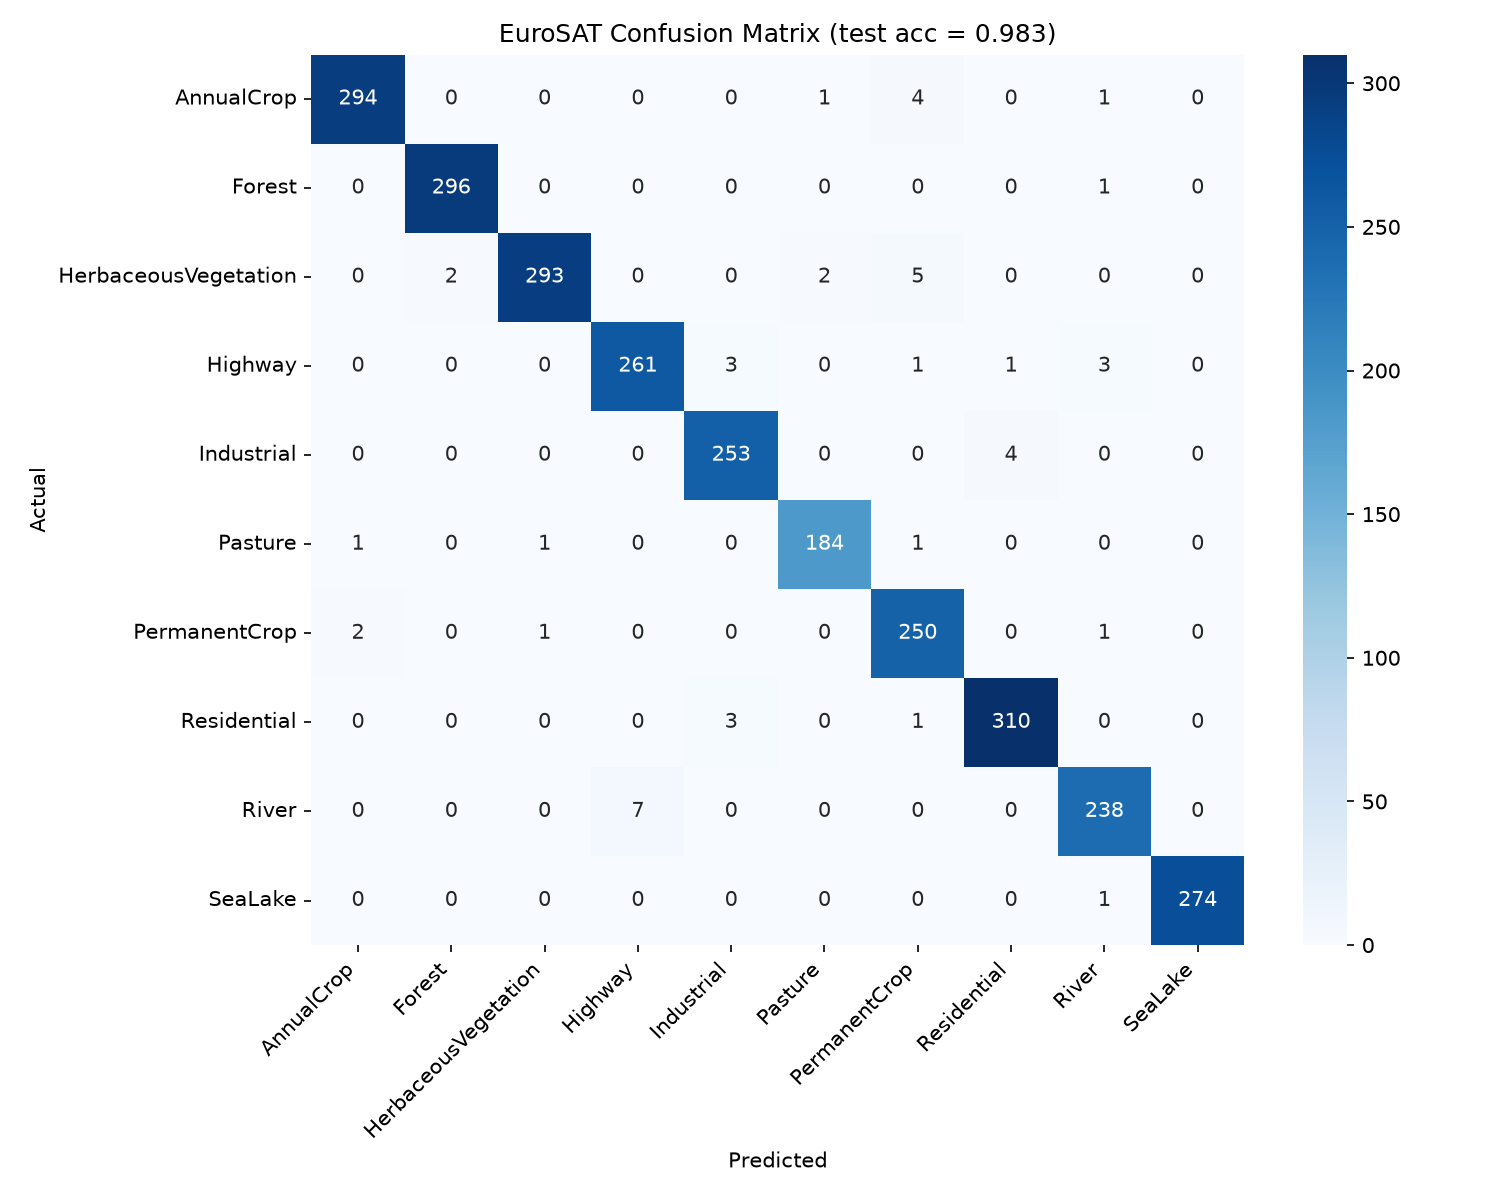
\includegraphics[width=\columnwidth]{confusion_matrix.png}
\caption{EuroSAT test-set confusion matrix (test accuracy 0.983).}
\label{fig:cm}
\end{figure}

\subsection{Controlled Domain-Adaptation Ablation}
We have no labeled Sentinel-2 ground truth, so we cannot measure adaptation on the
real target domain. We built a controlled substitute: a nonlinear radiometric
corruption (per-channel gamma, gain, offset, and haze, tuned to the measured
EuroSAT-to-L2A gap) applied to the labeled EuroSAT test set
(Table~\ref{tab:ablation}). Nonlinearity matters, since a per-channel linear method
could otherwise invert the shift and the comparison would prove nothing. An
unadapted classifier gives up 47 points. Moment matching, the pipeline's default,
recovers 28\% of that, and histogram matching recovers none. AdaBN recovers 99\%
without a single label, which is what sent us to test it on real scenes. Note that
the two matching conditions draw their reference statistics from the clean version
of the very images being scored, which is more information than either would have
in deployment; the leak flatters them, so AdaBN's margin is a floor.

\begin{table}[!t]
\caption{Adaptation on a controlled shift (EuroSAT test set, $n{=}2700$).}
\label{tab:ablation}
\centering
\begin{tabular}{lcc}
\toprule
Condition & Accuracy & Gap recovered \\
\midrule
Clean (upper bound) & 0.983 & n/a \\
Shifted, no adaptation & 0.514 & 0\% \\
Shifted, moment match & 0.647 & 28\% \\
Shifted, histogram match & 0.504 & $-2$\% \\
Shifted, \textbf{AdaBN} & \textbf{0.979} & \textbf{99\%} \\
\bottomrule
\end{tabular}
\end{table}

\subsection{Cross-Biome Detection: CNN vs AdaBN vs NDVI}
\label{sec:crossbiome}
We ran all three detectors at all eight sites against GFW
(Fig.~\ref{fig:multisite}, Table~\ref{tab:crossbiome}). The results do not support
a simple ``the CNN detects deforestation'' story.

\textbf{(a) The CNN is bimodal.} At three of eight sites it scores F1 $\leq$0.001.
Tshopo produces 46 detections of which one is correct (precision 0.022);
Mai-Ndombe and Gran Chaco produce none at all. The model labels most non-European
forest as something other than Forest, so it finds no Forest$\rightarrow$non-Forest
transitions to report. Both Congo sites fail independently on clean composites,
which makes this a systematic domain-shift failure rather than an artifact, and one
a single-site study would never surface. The same model then posts its best score
at Mato Grosso (F1 0.479, precision 0.574), a mechanized soy and pasture frontier
whose large rectangular clearings sit closest to EuroSAT's European domain. Strong
where the domain is near and absent where it is far: that split drives the CNN's sd
of 0.168, the widest of the three detectors.

\textbf{(b) AdaBN repairs every collapse.} Label-free BatchNorm adaptation lifts
all three zeros into positive territory. Tshopo goes from 0.001 to 0.397, with
precision climbing from 0.022 to 0.702 and 672 of 958 detections landing on real
loss; the CNN and AdaBN intervals ($[0.00,0.00]$ and $[0.37,0.43]$) do not overlap.
Mai-Ndombe goes from 0.000 to 0.198 and Gran Chaco from 0.000 to 0.100, and neither
of those intervals overlaps its CNN counterpart. Recovery quality varies by site. At
Tshopo the model recovers with its precision intact. At Mai-Ndombe it over-fires,
hitting 1{,}626 cells against 570 in the reference, so recall reaches 0.381 while
precision sits at 0.134. The model now sees forest and over-calls the change, which
is a different failure from seeing nothing, and a more tractable one.

\textbf{(c) AdaBN buys consistency.} It carries the lowest spread (sd
0.130) and never collapses, yet its mean F1 (0.250) trails NDVI's. On the easy
sites it moves little (Mato Grosso 0.479 to 0.486), and it costs a couple of points
at Riau and Santa Cruz. AdaBN pays off in proportion to how badly the domain has
shifted, which suggests gating the adaptation on a measured shift magnitude instead
of applying it always.

\textbf{(d) NDVI leads on average and still cannot be trusted alone.} It takes the
highest mean F1 (0.337), wins five of eight sites, and leads across the Amazon
(Mato Grosso 0.711), both Congo sites, and Gran Chaco. Then it falls apart at Santa
Cruz, returning 2 detections against 383 reference loss cells: both are correct,
giving a precision of 1.000 that means nothing next to a recall of 0.005. Its
dry-forest behavior is site-specific rather than biome-uniform, since it wins Gran
Chaco and loses Santa Cruz, where the compressed NDVI dynamic range defeats an
absolute 0.2-drop rule even with an adaptive threshold. On dry forest the two
families trade wins.

\textbf{What the statistics support.} Across eight sites the plain CNN trails NDVI
at the edge of significance ($p{=}0.055$). No other pair separates (AdaBN vs CNN
$p{=}0.31$, AdaBN vs NDVI $p{=}0.20$; per-site wins NDVI 5, CNN 2, AdaBN 1). Eight
sites give a signed-rank test little power, and we will not dress that up. The firm
results here are the per-site ones, where the block-bootstrap intervals separate
cleanly. We claim biome-dependence and robustness, and we do not claim a winning
method.

\begin{table}[!t]
\caption{Per-site F1 vs GFW (loss-frac $\geq$25\%), 95\% block-bootstrap CI.}
\label{tab:crossbiome}
\centering
\begin{tabular}{llccc}
\toprule
Site & Biome & CNN & CNN+AdaBN & NDVI \\
\midrule
Rond\^onia & Amazon & 0.234 & 0.242 & \textbf{0.495} \\
S\~ao F\'elix & Amazon & 0.232 & 0.229 & \textbf{0.304} \\
Mato Grosso & Amazon & 0.479 & 0.486 & \textbf{0.711} \\
Riau & Peat/palm & \textbf{0.248} & 0.222 & 0.177 \\
Tshopo & Congo & 0.001 & \textbf{0.397} & 0.220 \\
Mai-Ndombe & Congo & 0.000 & 0.198 & \textbf{0.384} \\
Santa Cruz & Dry forest & \textbf{0.156} & 0.126 & 0.010 \\
Gran Chaco & Dry forest & 0.000 & 0.100 & \textbf{0.392} \\
\midrule
mean $\pm$ sd & & 0.169 & 0.250 & \textbf{0.337} \\
              & & $\pm$.168 & $\pm$.130 & $\pm$.213 \\
\bottomrule
\end{tabular}
\end{table}

\begin{figure}[!t]
\centering
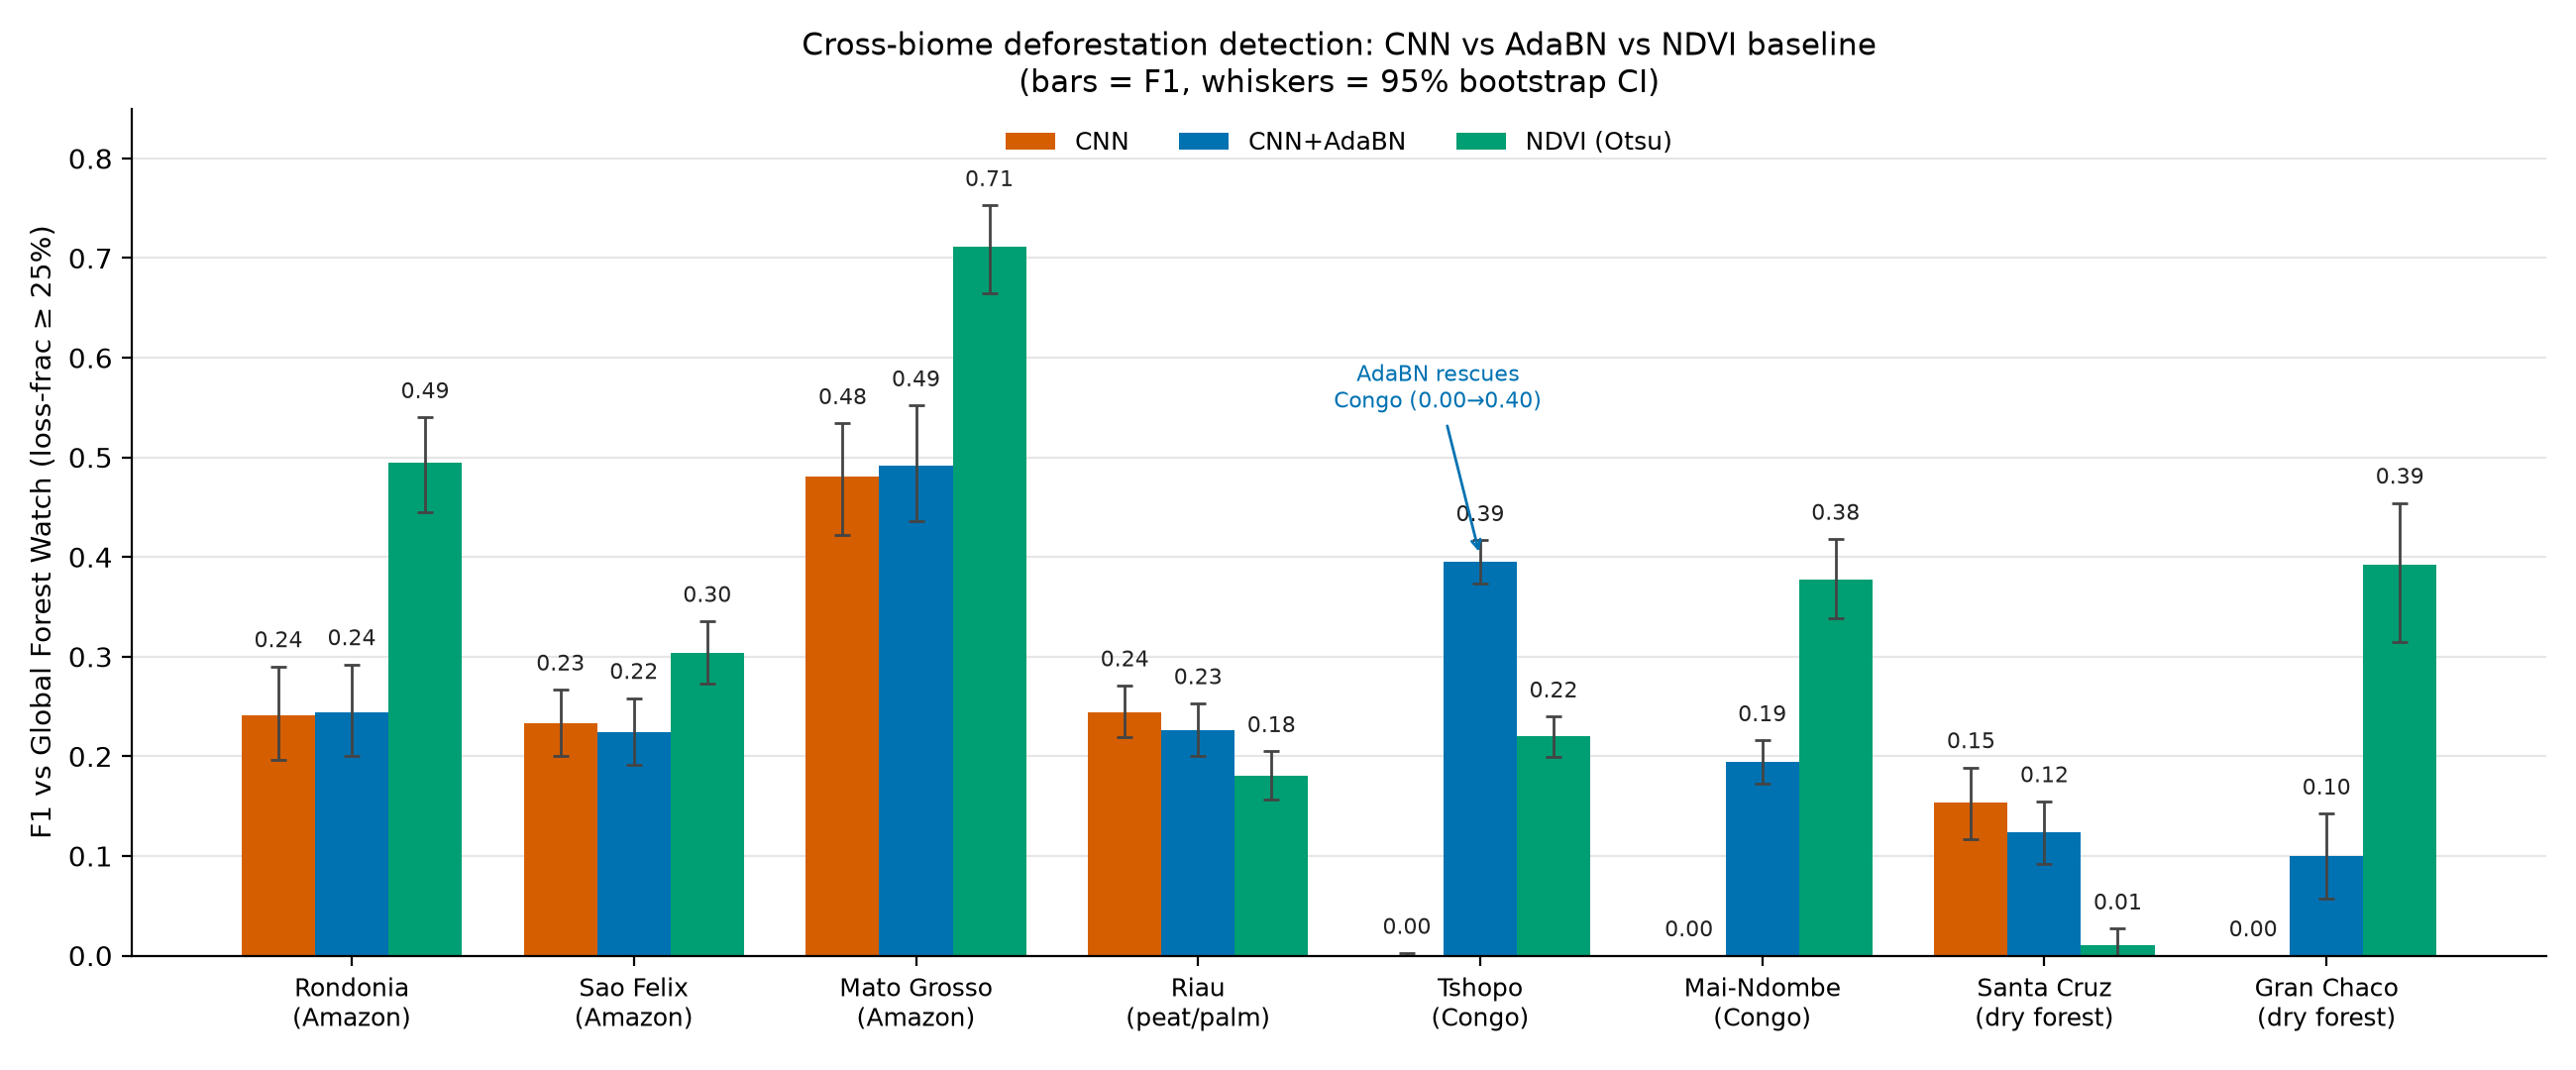
\includegraphics[width=\columnwidth]{multisite_f1_comparison.png}
\caption{Cross-biome F1 vs Global Forest Watch (loss-frac $\geq$25\%) for CNN,
CNN+AdaBN, and the NDVI baseline; whiskers are 95\% block-bootstrap CIs. AdaBN
rescues the Congo Basin site from F1 0.001 to 0.397.}
\label{fig:multisite}
\end{figure}

\begin{figure}[!t]
\centering
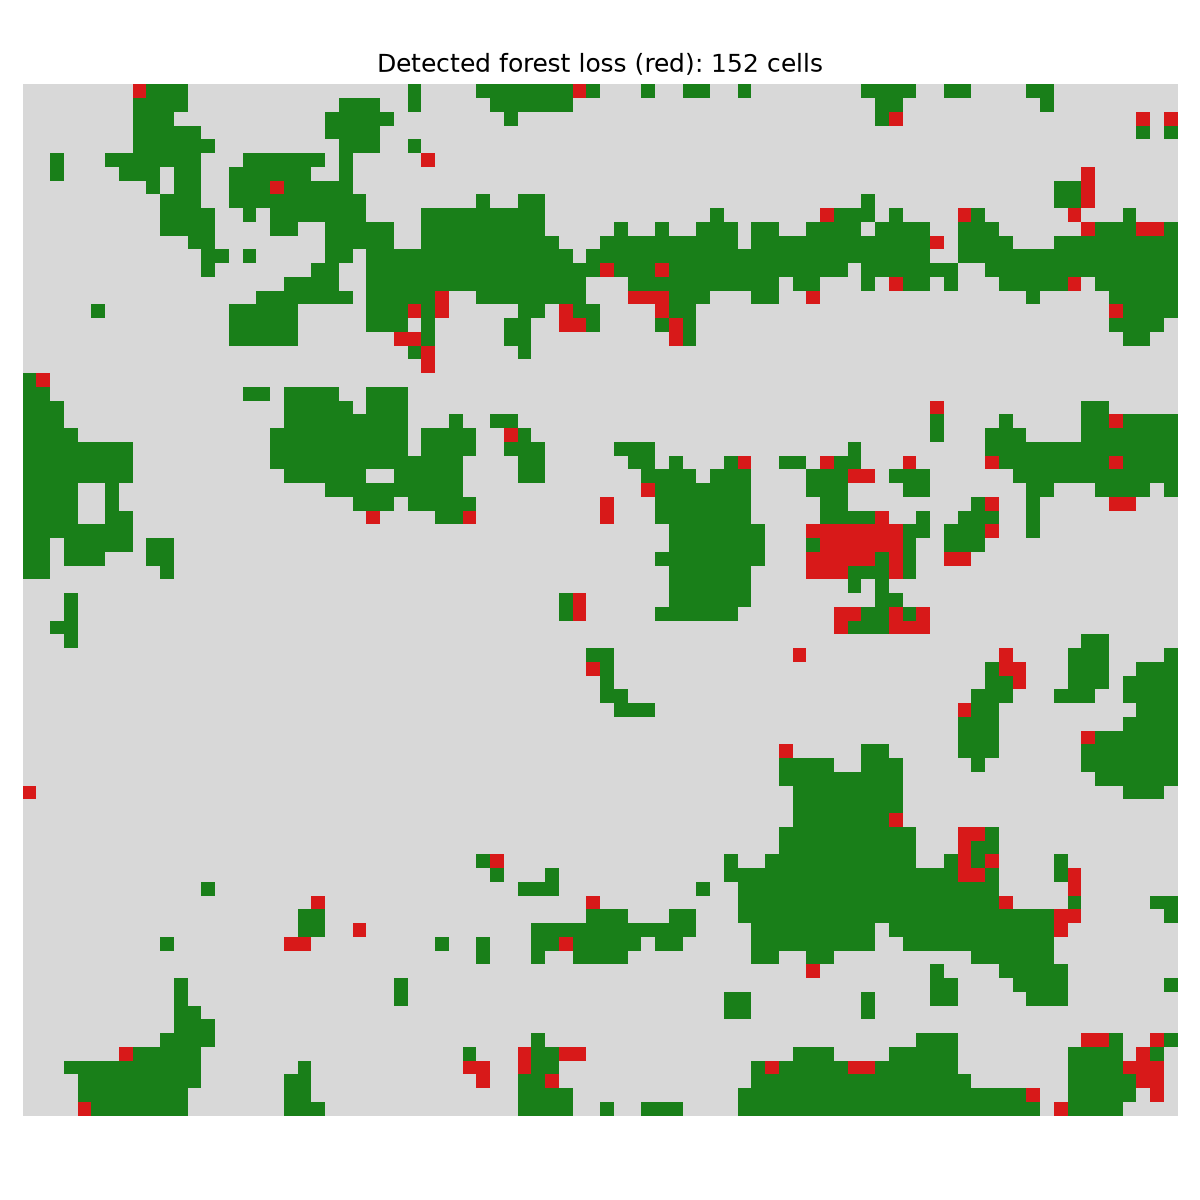
\includegraphics[width=\columnwidth]{rondonia_change_changemap.png}
\caption{Rond\^onia detected forest loss (red), 2016$\rightarrow$2024. Green:
forest retained; grey: non-forest.}
\label{fig:rond}
\end{figure}

\section{Discussion}
In-benchmark accuracy tells you little about cross-biome behavior. Our 98\%-accurate
classifier fails two ways once it leaves Europe. Uncorrected radiometry turns
rainforest into water and raises no error along the way. Then, at three of eight
sites, the model stops finding anything at all, and it does so at two Congo
frontiers that share nothing beyond a biome. Evaluating on one site would have
hidden both failures. We found them by taking the same model to eight sites and
looking for the breaks, which is also what made the repair testable.

The repair is cheap. AdaBN wants no labels, no retraining, and one forward pass,
and it clears every collapse while producing the steadiest detector we tested. For
an operational screening tool that trade is worth taking, because a blind spot
covering an entire biome costs more than a few points of mean F1 elsewhere. NDVI's
higher average does not change that.

The NDVI comparison keeps the CNN honest. A 1979 spectral index beats a fine-tuned
ResNet50 on mean F1 across our sites, and anyone proposing a CNN here owes that
baseline an answer. But the index breaks too, collapsing at one of the two
dry-forest sites while winning the other. The methods are complements: NDVI excels
where clearing leaves a strong spectral signature, and the adapted CNN is the safer
default where it does not.

\textbf{Limitations.} Eight sites limit across-site power, and more frontiers per
biome would sharpen the significance testing. A ninth site, Kalimantan, was acquired
and then excluded, because its only obtainable 2016 composite was cloud-degraded and
not radiometrically comparable to 2024. Patches of 640\,m miss small and linear
clearings, which caps recall against fine-grained GFW loss. The NDVI baseline uses an
absolute-drop rule, and a relative-drop variant might treat dry forest more fairly.
AdaBN adjusts only second-order statistics, so deeper shift goes unaddressed. Our
reference interval excludes Hansen loss labeled 2016, which charges a false positive
for any late-2016 clearing a detector catches. Finally, the pipeline classifies
tropical imagery with a model trained on European scenes; region-matched labels would
shrink the underlying shift instead of correcting for it after the fact.

\section{Conclusion}
A lightweight ResNet50/EuroSAT pipeline recovers a deforestation signal that agrees
with Global Forest Watch, but only inside its comfort zone. Across eight frontiers
it fails outright at three, and we trace that failure to domain shift and repair it
with a label-free AdaBN pass that leaves us with the most consistent detector across
three biomes. A classical NDVI baseline still posts the highest mean F1 and still
breaks at a site of its own. No detector dominates, and robustness across biomes
deserves more weight than peak in-biome F1. Five directions follow: add sites per
biome for statistical power; gate adaptation on a measured shift magnitude; push
past BatchNorm to feature alignment and region-matched fine-tuning; move to finer
patches or segmentation for sub-patch clearings; and swap the two-snapshot design
for multi-temporal sequences.

\begin{thebibliography}{11}
\bibitem{hansen2013} M.~C. Hansen \emph{et al.}, ``High-Resolution Global Maps of 21st-Century Forest Cover Change,'' \emph{Science}, vol.~342, no.~6160, pp.~850--853, 2013.
\bibitem{curtis2018} P.~G. Curtis \emph{et al.}, ``Classifying drivers of global forest loss,'' \emph{Science}, vol.~361, no.~6407, pp.~1108--1111, 2018.
\bibitem{fao2020} FAO, \emph{Global Forest Resources Assessment 2020}, Rome, 2020.
\bibitem{helber2019} P.~Helber, B.~Bischke, A.~Dengel, D.~Borth, ``EuroSAT: A Novel Dataset and Deep Learning Benchmark for Land Use and Land Cover Classification,'' \emph{IEEE JSTARS}, vol.~12, no.~7, pp.~2217--2226, 2019.
\bibitem{he2016} K.~He, X.~Zhang, S.~Ren, J.~Sun, ``Deep Residual Learning for Image Recognition,'' in \emph{CVPR}, 2016.
\bibitem{deng2009} J.~Deng \emph{et al.}, ``ImageNet: A Large-Scale Hierarchical Image Database,'' in \emph{CVPR}, 2009.
\bibitem{drusch2012} M.~Drusch \emph{et al.}, ``Sentinel-2: ESA's Optical High-Resolution Mission for GMES Operational Services,'' \emph{Remote Sens. Environ.}, vol.~120, pp.~25--36, 2012.
\bibitem{li2016} Y.~Li, N.~Wang, J.~Shi, J.~Liu, X.~Hou, ``Revisiting Batch Normalization for Practical Domain Adaptation,'' arXiv:1603.04779, 2016.
\bibitem{ioffe2015} S.~Ioffe, C.~Szegedy, ``Batch Normalization: Accelerating Deep Network Training by Reducing Internal Covariate Shift,'' in \emph{ICML}, 2015.
\bibitem{otsu1979} N.~Otsu, ``A Threshold Selection Method from Gray-Level Histograms,'' \emph{IEEE Trans. Syst., Man, Cybern.}, vol.~9, no.~1, pp.~62--66, 1979.
\bibitem{tucker1979} C.~J. Tucker, ``Red and Photographic Infrared Linear Combinations for Monitoring Vegetation,'' \emph{Remote Sens. Environ.}, vol.~8, no.~2, pp.~127--150, 1979.
\end{thebibliography}

\end{document}
